\newpage
\subsection{Теорема о локальном диффеоморфизме}
\begin{theorem} (Теорема Лагранжа о среднем).
    Пусть отображение $F \in \DIF(B_\delta (x^0) {\scriptstyle \subset \R^m},\ \R^n)$. Тогда $\forall y, z \in B_\delta (x^0)\; \exists \theta \in (0, 1)$:

$$\|F(y) - F(z)\| \leqslant \|\D F(y + \theta(z - y)\| \|y - z\|$$
\end{theorem}
\begin{proof}
Так как шар~---~выпуклое мн-во, то $[y, z] = \{x = y + t(z - y) : t \in [0, 1]\} \subset B_\delta(x^0)$.\\
Рассмотрим отображение $f(t) = F(y + t(z - y))$. Получим отображение $f$: $[0, 1] \mapsto \R^n$.
По теореме о композиции дифференцируемого отображения, $f$ является дифференцируемым отображением и $f'(t) = \D F(y + t(z - y)) \cdot (z - y)$ 
По теореме Лагранжа о среднем для функции $f$ $\exists \theta \in (0, 1)$:

$$\|F(y) - F(z)\| = \|f(1) - f(0)\| \leqslant \|f'(\theta)\|(1 - 0) = \|\D F(y + \theta(z - y))(z - y)\| \leqslant \|\D F(y + \theta(z - y))\| \|z - y\|.$$
\end{proof}
\begin{definition}
    $J_F(x^0) := \det \D F(x^0)$, называется \textit{Якобиан}.
\end{definition}
\begin{theorem}[о локальной обратимости отображений/диффеоморфизме]

    Пусть $F \in C^1(\Omega, \R^m)$, $\Omega \subset \R^m$, $J_F(x^0) \neq 0$, где $x^0 \in \Omega$. Тогда $\exists U \subset \Omega$: $U \ni x^0$, F осуществляет диффеоморфизм $U$ на $F(U)$.
\end{theorem}
\begin{proof}
    Так как $J_F(x^0) \neq 0 \Longleftrightarrow \text{обратимость отображения } \D F(x^0) \implies \exists$ <<малый>>\ шар $B_{\delta_1}(x^0)$:
    $J_F(x) \neq 0 \quad \forall x \in  B_{\delta_1}(x^0)$. \\
    Так как $\D F(x^0)$ обратима, то $\|\D F(x^0)x\| \geqslant \|\D F(x^0)^{-1}\| \|x\|$. Пусть $c := \|\D F(x^0)^{-1}\|$.
    Так как $F \in C^1(\Omega, \R^m)$, то матрица Якоби непрерывна как функция точки $x$.

    \begin{equation}
        \implies \exists \delta_2 > 0: \forall x \in B_{\delta_2}(x^0) \hookrightarrow \|\D F(x^0) - \D F(x)\| < \frac{c}{2}.
        \label{eq:locdiff_proof1}
    \end{equation}

    $\delta = \min\{\delta_1, \delta_2\}$.
Покажем, что отображение $F$ инъективно в $B_\delta(x^0)$.
\begin{flushleft}
    $\|F(x) - F(y)\| = \| F(x) - F(y) - \D F(x^0)(x - y) + \D F(x^0)(x - y)\| \geqslant $
\end{flushleft}
\begin{flushright}
    $\geqslant \|\D F(x^0)(x-y)\| - \|F(x) - F(y) - \D F(x^0)(x - y)\|$
\end{flushright}


Применим теореме Лагранжа о среднем к отображению $L(x) = F(x) - \D F(x^0) \cdot x$
\[
    \|L(x) - L(y)\| = \|F(x) - F(y) - \D F(x^0)(x - y)\|
\]
\[
    \|L(x) - L(y)\| \leqslant \|L'(x + \theta(y - x))\| \|y - x\| = \|\D F(x + \theta(y - x)) - \D F(x^0)\| \|y - x\|
\]

Но по \eqref{eq:locdiff_proof1} $\|\D F(x + \theta(y - x)) - \D F(x^0)\| \leqslant \frac{c}{2}$, то есть $\|L(x) - L(y)\| \leqslant \frac{c}{2}\|y - x\|$

Вернёмся к \eqref{eq:locdiff_proof2}. Мы показали, что $\|F(x) - F(y) - \D F(x^0)(x - y)\| \leqslant \frac{c}{2}\|y - x\|$, при этом по обратимости $\D F(x^0)$, $\|\D F(x^0)(x-y)\| \geqslant c\|x - y\|$

Итого,
\begin{equation}
\begin{split}
    \|F(x) - F(y)\| \geqslant c\|x - y\| - \frac{c}{2}\|x - y\| = \frac{c}{2}\|x - y\| \\
    \implies F(x) \neq F(y) \forall x, y \in B_\delta(x^0) \\
    \implies F - \text{инъективно на } B_\delta(x^0)
\end{split}
\end{equation}

Но $J_F(x) \neq 0\; \forall x \in B_\delta(x^0)$ и $F \in C^1(B_\delta(x^0), \R^m) \implies $ работают все условия теоремы об открытом отображении и об обратном отображении. Мы доказали инъективность, значит есть обратное

$\exists F^{-1} : F(B_\delta(x^0) {\scriptstyle \subset \R^m, \text{открытое множество}}) \mapsto B_\delta(x^0)$

$\implies$ по теореме об обратном отображении F - диффеоморфизм $B_\delta(x^0)$ на $F(B_\delta(x^0))$
\end{proof}
\begin{note}
    Может оказаться так, что $F\in C^1(\Omega, \R^m)$.

    $J_F(x) \neq 0 \; \forall x \in \Omega$

    Но на всём $\Omega$ отображение F не является инъективным $\implies$ не является глобально обратимым

    \begin{example}
        \[
        F(x, y) =
        \begin{pmatrix}
            e^x \cos y \\
            e^x \sin y
        \end{pmatrix}
        \]
        очевидно $F \in C^1(\R^2, \R^2)$

        \[
        J_F(x, y) = \det
        \begin{pmatrix}
            e^x \cos y & -e^x \sin y \\
            e^x \sin y & e^x \cos y
        \end{pmatrix}
        = e^x > 0 \quad \forall (x, y) \in \R^2
        \]
        Но при этом $(x, y) \text{ и } (x, y + 2\pi)$ переходят в одну и ту же точку.
    \end{example}
\end{note}

\subsection{Продолжение отображения до диффеоморфизма}
\newcommand{\Fover}{\overline{F}}
$\R^m$ будем отождествлять с подпространством в $R^n$, образованного векторами \\ 
$(x_1, \hdots, x_m, 0, \hdots, 0)$ \\
$\R^m \equiv \R^m \times \{0\} \; \subset \R^n$ \quad \quad (тут имеется в виду $0\ (n - m)$-мерного пространства)

\begin{theorem}
    Пусть выполнены следующие условия:
    \begin{itemize}
        \item $F \in C^1(\Omega {\scriptstyle \subset \R^m}, \R^n)$
        \item $n > m$. Пусть $\rank \D F(x^0) = m$, $x^0 \in \Omega$. 
    \end{itemize}

    Тогда $\exists n-\text{мерная окрестность } V \text{ точки } (x^0, 0) \in \R^n$ и отображение $\Fover$ является диффеоморфизмом $V$ на $\Fover(V), \text{где } \Fover|_{V \cap \R^m} := F$. 
\end{theorem}
\begin{proof}
    Так как $\rank \D F(x^0) = m \implies $ есть подматрица $m\times m$ с ненулевым определителем.

    Без ограничения общности считаем, что матрица $m\times m$ образована первыми $m$-строками и $m$-координатами.

    $\R^n = (x, y), \text{ где } x \in \R^m, y \in \R^{n-m}$

    $U = \Omega \times \R^{n - m}$

    $\Fover(x, y) = F(x) + \begin{pmatrix} 0 \\ y \end{pmatrix}$\quad заметим, что $\Fover|_U = F$
  
    $\D \Fover(x, y) = \D F(x) + \begin{pmatrix} 0 \\ E \end{pmatrix} \implies \D \Fover(x^0, 0)$~---~обратима

    $\implies \text{ к } \Fover$ применима теорема о локальном диффеоморфизме, то есть $\exists V \subset \R^n, V \ni (x^0, 0)$: $\Fover$ осуществляет диффеоморфизм $V$ на $\Fover(V)$.
\end{proof}

\newpage
\subsection{Теорема о неявной функции}

\begin{center}
$\R^{n+m} = \R^m \times \R^n$

$c_i \in \R, i \in \{1, \hdots, n\}$
\end{center}
Рассмотрим систему уравнений, мы хотим уметь решать ее, при каждом фиксированном x, относительно y. То есть x играет роль параметра, и мы решаем систему:
\begin{center}

\begin{equation}
\begin{split}
    &\begin{cases}
        F_1(x_1, \hdots, x_m, y_1, \hdots, y_n) = c_1 \\
        \vdots \\
        F_n(x_1, \hdots, x_m, y_1, \hdots, y_n) = c_n \\
    \end{cases}
    \\
    &F(x, y) = c
\end{split}
\label{eq:for_implicit}
\end{equation}
\end{center}

Предположим, что при каждом значении x, мы нашли единственный y. Тогда мы получили фцнкцию от x. Такую функцию мы будем называть неявной

\begin{definition}
    Пусть $F$: $E \mapsto \R^n, \text{ где } E \neq \varnothing, E \subset \R^{n+m}$. Будем говорить, что отображение $f$: $X \mapsto \R^n$ явл. неявным отображением, заданным уравнением \eqref{eq:for_implicit}, если $\begin{cases}
        (x, f(x)) \in E \quad \forall x \in X \\
        F(x, f(x)) \equiv 0 \text{ на } X
    \end{cases}$
\end{definition}
\begin{definition}
    Множеством уровня функции, будем называть множество тех точек, где её значение постоянно
\end{definition}

\begin{example}
    $x^2 + y^2 = 1$

    Окружность, которую задаёт это уравнение~---~это множество уровня отображения $x^2 + y^2$.

    $y(x)$ может быть как $\sqrt{1 - x^2}$, так и $-\sqrt{1 - x^2}$, и $(2\D(x) - 1)\sqrt{1 - x^2}$($\D(x)$~---~ функция Дирихле). Это всё функции заданные неявно этим уравнением. Причина состоит в том, что при каждом $x$ есть 2 решения, поэтому число выборов этих функций очень большое.

    Функция единственна, когда множество уровня является графиком функции, и оказывается говорить об этом можно только в локальной окрестности. Если пересечь окружность с малой окрестностью, то локально множество уровня будет выглядеть как график. Это и есть теорема о неявном отображении или о неявной функции (неформально), сейчас мы её аккуратно сформулируем.
\end{example}
\begin{theorem}
    (о неявном отображении) Пусть $F \in C^1 (G{\scriptstyle \subset \R^{n + m}}, \R^n)$
    Если выполены следующие условия:
    \begin{enumerate}
        \item $F(x^0, y^0) = 0$
        \item $\det \D_y F(x^0, y^0) \neq 0$
    \end{enumerate}
    
    \[
    \D F = 
    \begin{pmatrix}
        \frac{\partial F_1}{\partial x_1} & \cdots & \frac{\partial F_1}{\partial x_m} & \frac{\partial F_1}{\partial y_1} & \cdots & \frac{\partial F_1}{\partial y_n} \\
        \vdots \\
        \frac{\partial F_n}{\partial x_1} & \cdots & \frac{\partial F_n}{\partial x_m} & \frac{\partial F_n}{\partial y_1} & \cdots & \frac{\partial F_n}{\partial y_n} \\ 
    \end{pmatrix}
    = (\D _x F , \ \D _y F)
    \]

    (Правую часть этой матрицы и назовём $\D_y F$)

    \[ \text{Тогда }
    \begin{cases}
    \exists U(x^0) \subset \R^m \\
    \exists V(y^0) \subset \R^n \\
    \end{cases}
    \text{такие, что } \forall x^* \in U(x^0)\; \exists! y^*\in V(y^0): F(x^*, y^*) = 0
\]

    $\Longleftrightarrow$ м-во нулей отображения $F$, пересечённое с $U\times V$ имеет вид графика некоторого отображения $f: U \mapsto V$

    При этом, $f \in C^1(U, V)$ и $\D_x f(x^0) = -(\D_y F(x^0, y^0))^{-1} (\D_x F(x^0, y^0))$
\end{theorem}
\begin{proof}
    Сведём всё к теореме о локальном диффеоморфизме. \\
    \[ \text{Для этого введем вспомогательное отображение }
    \begin{cases}
    \Phi: G \mapsto \R^{m+n} \\
    \Phi(x, y) \stackrel{\Phi}{\longrightarrow} (x, F(x, y))
    \end{cases}
    \]

    Заметим, $\D \Phi (x^0, y^0) = \begin{pmatrix}
        E_{m\times m} & 0 \\
        \D_x F & D_y F \\
    \end{pmatrix} \implies \det \D \Phi(x^0, y^0) \neq 0$ и $\Phi \in C^1(G, \R^{m + n})$ \\
    Значит применима теорема о локальном диффеоморфизме для $\Phi \Longrightarrow \ \exists$ окрестность $W$ точки $(x^0, y^0)$: $\Phi$ осуществляет диффеоморфизм $W$ на $\Phi(W)$.


    Рассмотрим $\Phi(x^0, y^0) \stackrel{\Phi}{\longrightarrow} (x^0, 0)$. Геометрический смысл этого~---~распрямление множества нулей
    
    % \begin{wrapfigure}{R}{0.5\textwidth}
    %     \centering
    %     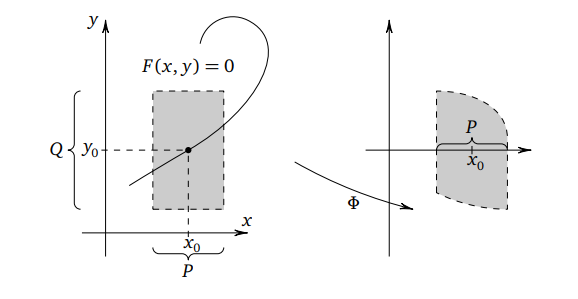
\includegraphics[width=0.47\textwidth]{Pictures/implicit}
    % \end{wrapfigure}

    Так как $\Phi(W)$~---~открыто, то $\exists \delta > 0\; \exists \epsilon > 0: B_\delta(x^0)\times B_\epsilon(0) \subset \Phi(W) \quad \forall x \in B_\delta(x^0)$

    Так как $\Phi$ взаимно однозначно, каждая точка из $\Phi(W)$ пришла из единственной точки из множества нулей. И имеет вид $(x, y) \stackrel{\Phi}{\longrightarrow} (x, 0)$

    $$\forall x \in \Phi(W) \cap \R^m \quad \exists! y \in \text{ м-ва нулей } F(x, y): \ F(x, y) = 0.$$
    $\implies$ Получили отображение $f$: $x \longrightarrow y$, как решение уравнения $F(x, y) = 0$.

    В итоге: 
    $\exists \delta > 0 \; \exists \epsilon > 0$ т. ч. $\forall x \in B_\delta(x^0) \; \exists! y \in B_\epsilon(y^0)$ т.ч. $F(x, y) = 0 \implies$

    \begin{equation}
        \implies F(x, f(x)) \equiv 0 \text{ на } B_\delta(x^0)
        \label{eq:for_implicit2}
    \end{equation}


    Тогда мы понимаем как выглядит обратное отображение $\Phi^{-1}(x, 0) = (x, f(x))$. Тк оно должно точку $(x, 0)$ возвращать в какой-то $(x, \hat{y})$, но $f(x) = \hat{y}$, по построению

    Но $\Phi^{-1}$ диффеоморфизм $\implies \Phi^{-1}$ является гладким отображением, $\Phi^{-1} \in C^1(\Phi(W), W)$

    $\implies f \in C^1(B_\delta(x^0), B_\epsilon(y^0))$

    Мы доказали гладкость, чтобы найти производную, продифференцируем \eqref{eq:for_implicit2} по $x$ на $B_\delta(x^0)$:

    $\D_x[F(x, f(x))] = (\D_x F)(x, f(x)) + \D_y F(x, f(x)) \cdot \D_x f \equiv 0$ 
    

    $$\implies \D_x f(x^0) = -\D_y F(x^0, y^0)^{-1}\cdot \D_x F(x^0, y^0)$$
\end{proof}